\pagebreak

\section{Proposed OHGesture Model}
\label{sec:ohgesture}

\begin{figure}[H]
	\centering
		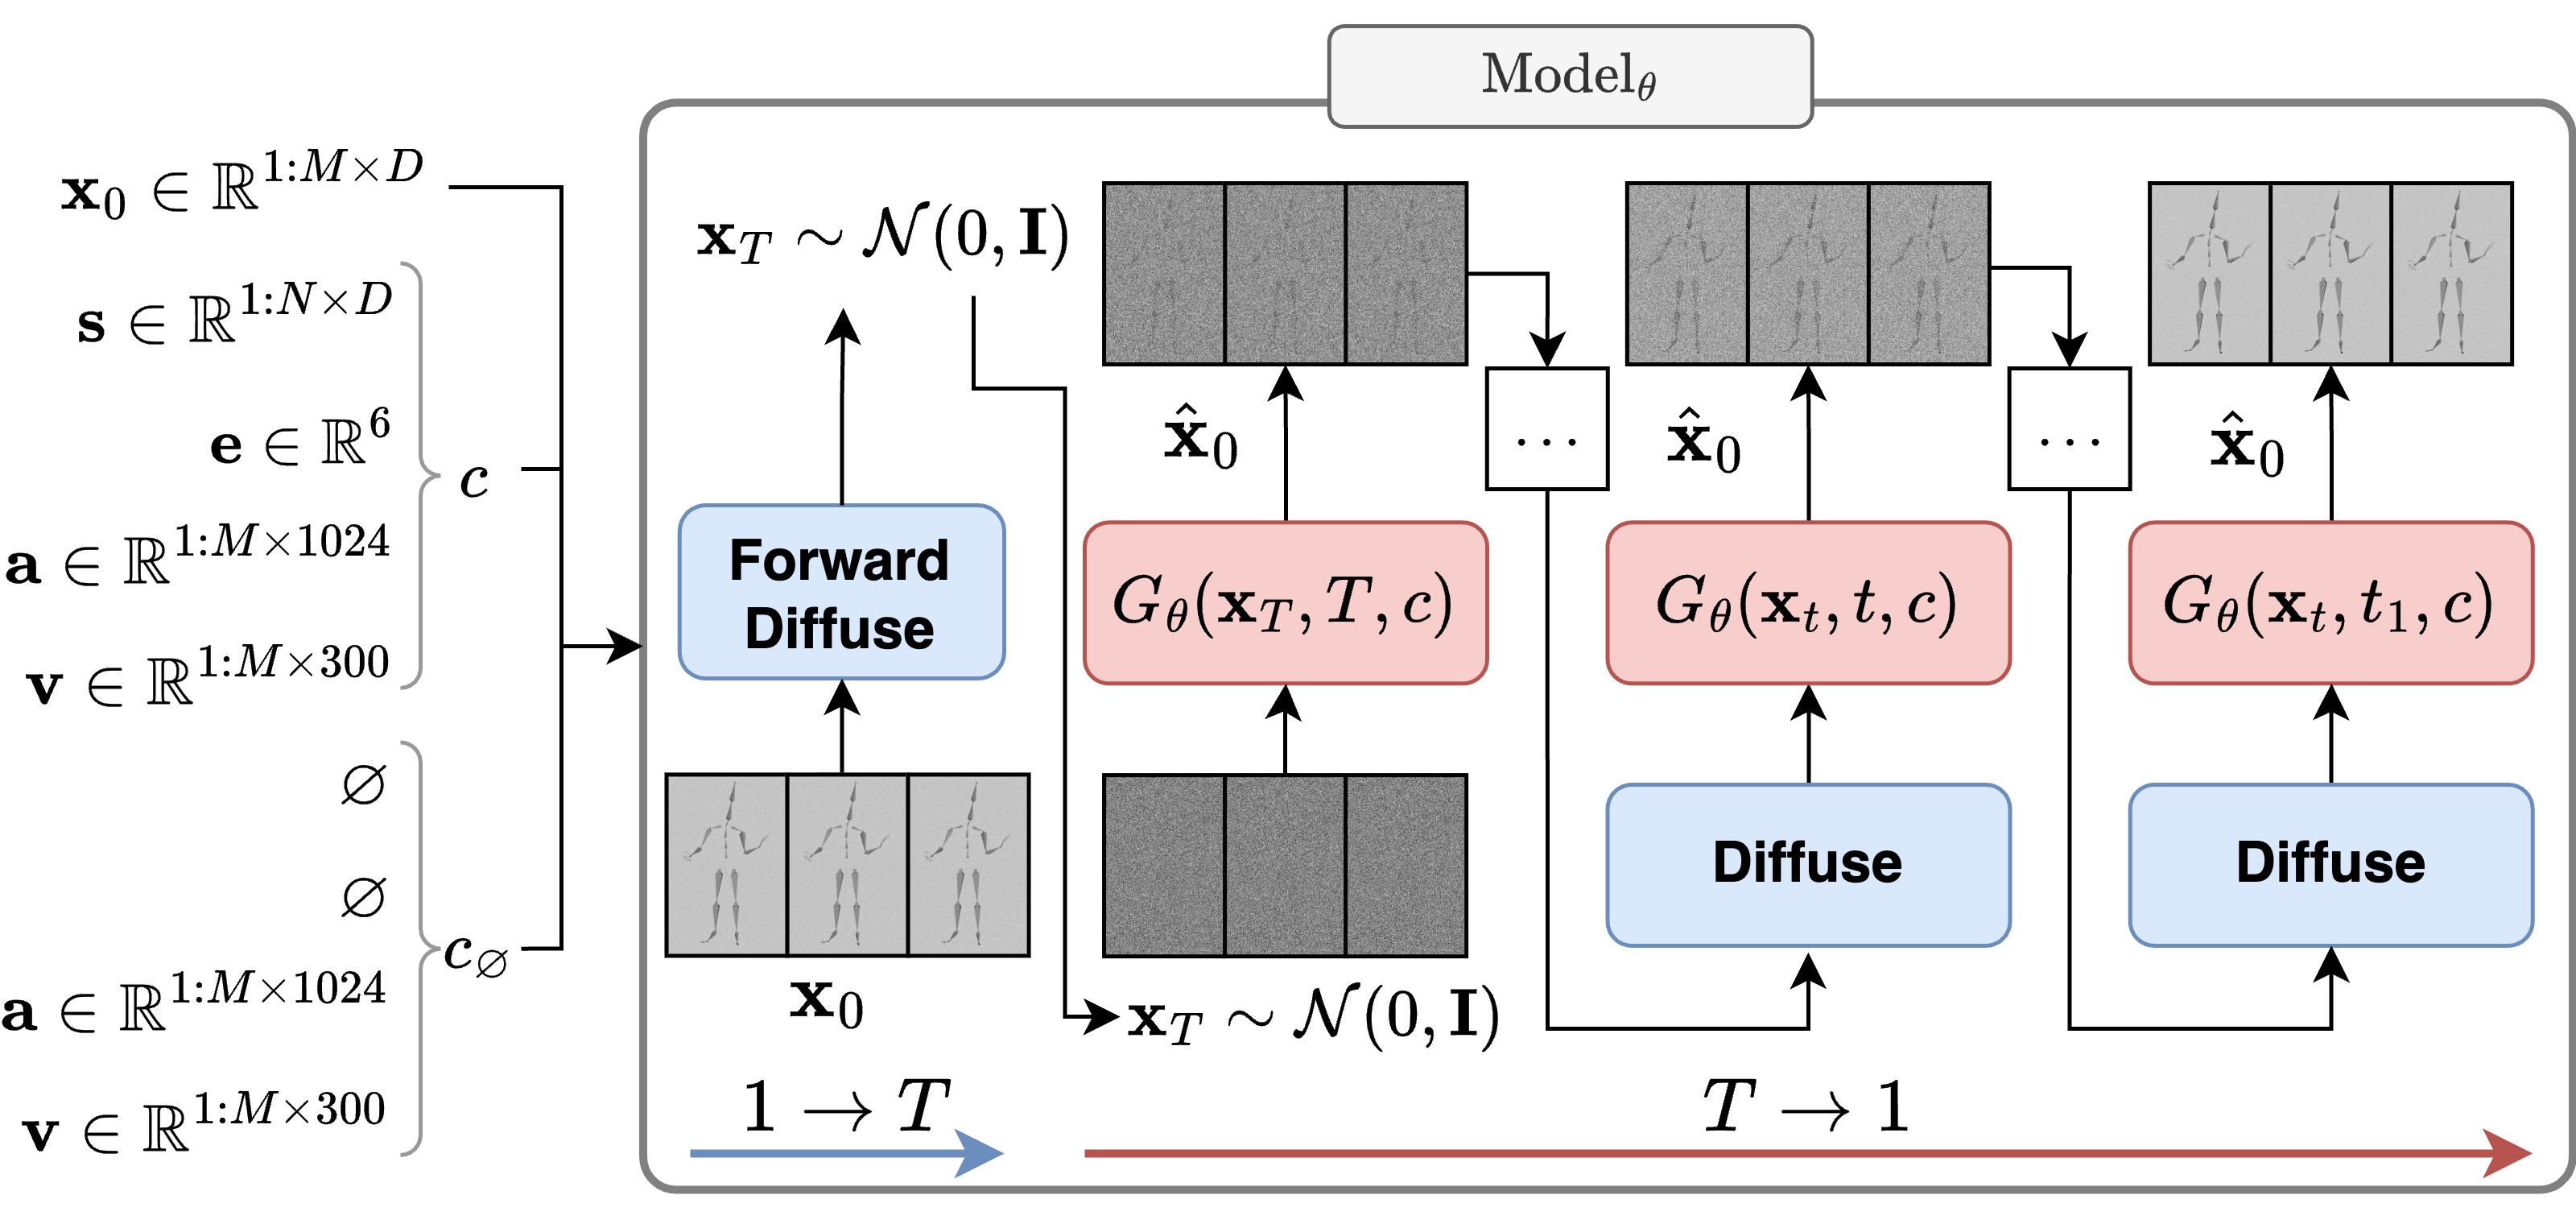
\includegraphics[width=\linewidth]{AllStage}
	\caption{Overview of the OHGesture model}
	\label{fig:TrainingAndSampling}
\end{figure}

The proposed model \textbf{OHGesture} (\textbf{O}pen \textbf{H}uman \textbf{Gesture} Generation) in this thesis is based on the \textbf{DiffuseStyleGesture} model \cite{yang2023diffusestylegesture}, which applies the Diffusion model \cite{ho2020denoising} with conditional guidance \cite{ho2022classifier} (Classifier-Free Diffusion Guidance) to control features during the denoising process.

The similarities and differences of applying the diffusion model to the gesture generation task compared to image generation are as follows:

\vspace{10pt}

\textbf{Similarities}
\begin{itemize}
	\item Uses the Diffusion model (\autoref{sec:summary_diffusion}) on gesture data $\bx^{1:M \times D}$, with $M$ temporal frames and $D=1141$ representing motion coordinates per frame (analogous to image width and height).
	\item Uses conditional Diffusion (\autoref{subsec:DiffusionCondition}) with $\bx_0$ objective (\autoref{subsec:X0Objective}).
	\item In stages \textit{4. Feature Encoding} and \textit{6. Feature Decoding} in \autoref{fig:CommonStage}, the model uses a latent vector of dimension $256$.
\end{itemize}

\textbf{Differences}
\begin{itemize}
	\item Conditional gesture generation:
	\begin{itemize}
		\item Emotional condition: $c = \big[ \mathbf{s}, \mathbf{e}, \mathbf{a}, \mathbf{v} \big]$ and $c_{\varnothing} = \big[ \varnothing, \varnothing, \mathbf{a}, \mathbf{v}\big]$.
		\item Emotion state interpolation between $\mathbf{e}_1, \mathbf{e}_2$ using: $c = \big[ \mathbf{s}, \mathbf{e}_1, \mathbf{a}, \mathbf{v} \big]$ and $c_{\varnothing} = \big[ \mathbf{s}, \mathbf{e}_2, \mathbf{a}, \mathbf{v} \big]$.
	\end{itemize}
	\item In stage \textit{5. Feature Fusion} \autoref{fig:CommonStage}, the model uses Self-Attention: learning the relationship between emotions, seed gestures, and each frame (similar to DALL-E 2's text-image alignment).
	\item In stage \textit{5. Feature Fusion} \autoref{fig:CommonStage}, the model concatenates speech and text (analogous to ControlNet's pixel-wise condition).
\end{itemize}

Here, $\bx_0$ is a sequence of $M$ gesture frames $\mathbf{x} \in \mathbb{R}^{1:M \times D}$ ($D = 1141$), with condition $c = [\mathbf{s}, \mathbf{e}, \mathbf{a}, \mathbf{v}]$ including seed gesture $\mathbf{s}$, emotion $\mathbf{e}$, speech $\mathbf{a}$ corresponding to the gesture, and text $\mathbf{v}$.

The model's objective is to learn parameters $\theta$ of the generative function $G_{\theta}$ with inputs being the noisy gesture matrix $\bx_t \in \mathbb{R}^{1:M \times D}$, timestep $t$, and condition $c$. An overview of the proposed \textbf{OHGesture} model is illustrated in \autoref{fig:TrainingAndSampling}. As with standard diffusion models, it includes two processes: the diffusion process $q$ and the denoising process $p_{\theta}$ with weights $\theta$. The \textit{1. Preprocessing} stage will be presented in \autoref{sec:Preprocessing}.


% (\operatorname{Query}) (\operatorname{Key}) (\operatorname{Value})
Cross-local Attention is performed with $\mathbf{Q} = \mathbf{K} = \mathbf{V} = \mathbf{m}_{t}$.
Following the idea of the Routing Transformer method \cite{roy2021efficient}, Cross-local Attention highlights the importance of constructing intermediate feature-vector representations before passing them through the Transformer Encoder layer, as shown in \autoref{fig:OHGesture}.
The feature vectors are augmented with a relative position-encoding vector \textbf{RPE} (\textbf{R}elative \textbf{P}osition \textbf{E}ncoding) to preserve temporal ordering before entering the Cross-Local Attention layer.

After Cross-Local Attention, the model is forwarded through a linear layer, as in \autoref{eq:CrossLocalAttention}, to align with the $M$ frames and obtain the matrix $\mathbf{h}_t \in \mathbb{R}^{1:M \times D}$.

\subsubsection{Global Feature Fusion with the Transformer Encoder}

\begin{figure}[H]
	\centering
	\begin{subfigure}{0.42\textwidth}
		\centering
		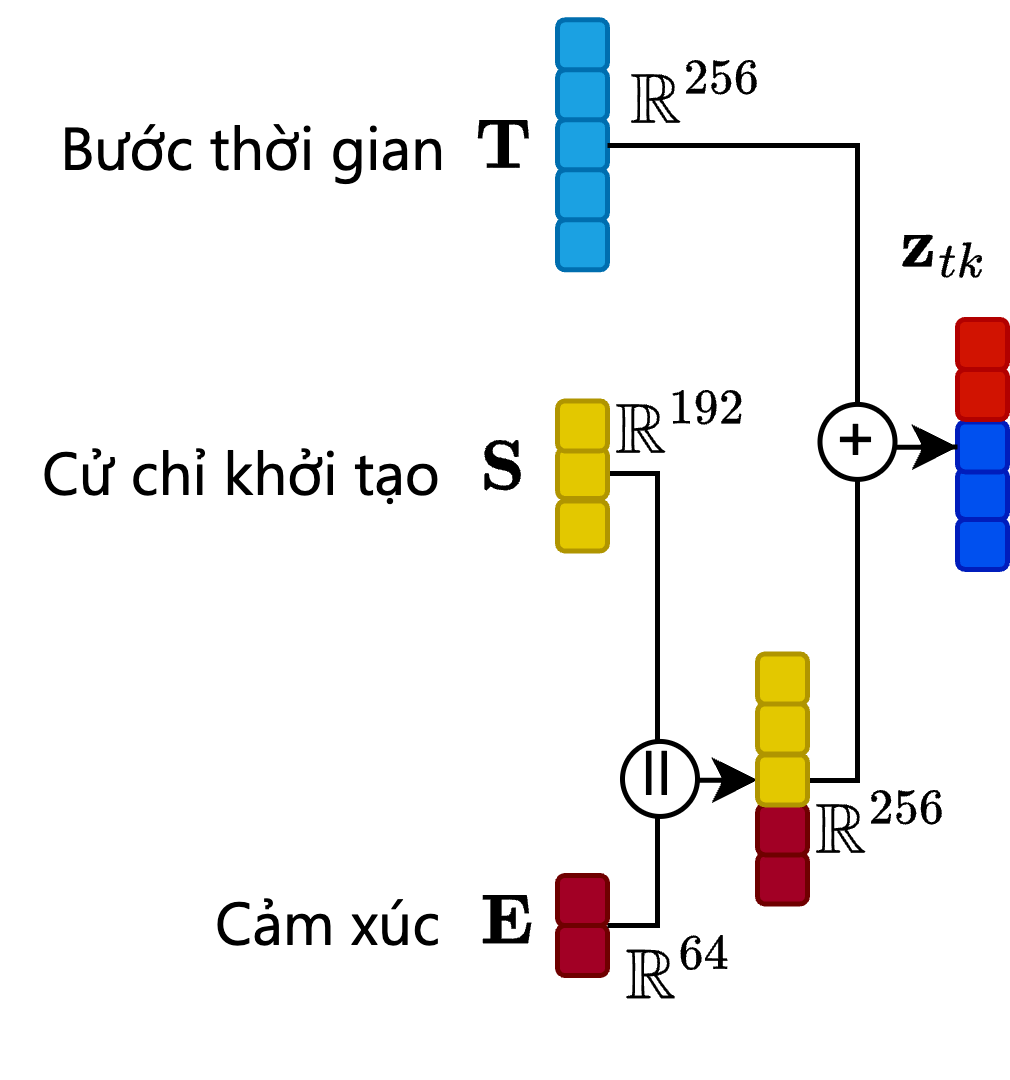
\includegraphics[width=0.9\textwidth]{z}
		\caption{How to concatenate features to obtain $\mathbf{z}_{tk}$}
		\label{fig:FeatureFusion}
	\end{subfigure}
	\hfill
	\begin{subfigure}{0.55\textwidth}
		\centering
		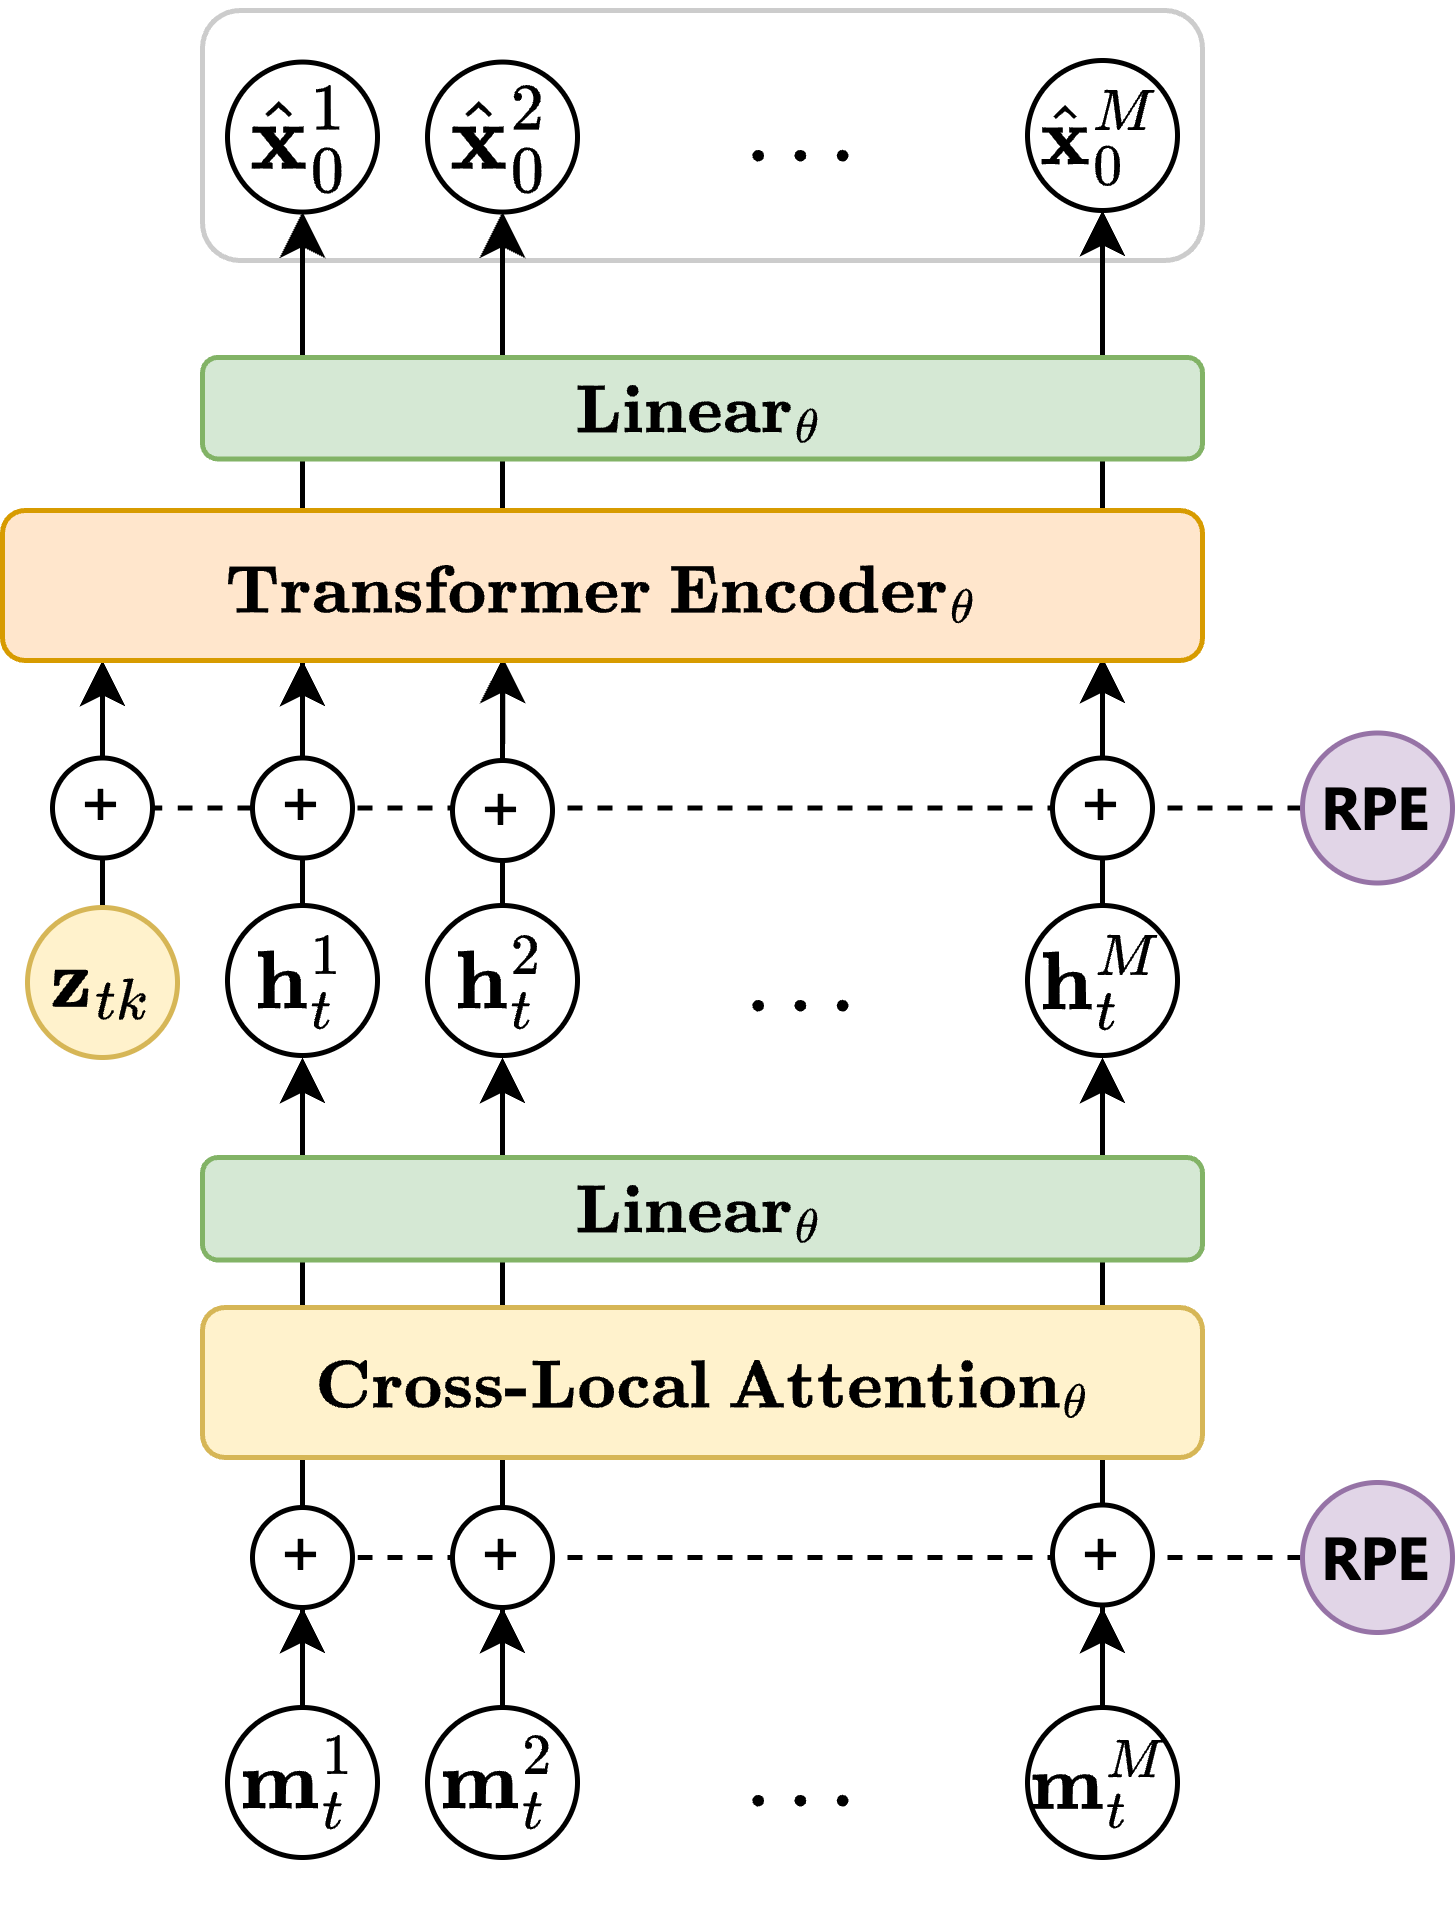
\includegraphics[width=0.85\textwidth]{FeatureFusion}
		\caption{Frame-wise feature-fusion process}
		\label{fig:ZToken}
	\end{subfigure}
\end{figure}

Following MDM \cite{tevet2022human}, the vector $\mathbf{z}_{tk}$ is the first token that encodes information for the entire frame sequence, analogous to the $\texttt{CLS}$ token in BERT \cite{devlin2019bertpretrainingdeepbidirectional}, which summarizes an entire text segment.
Here, the thesis uses $\mathbf{z}_{tk}$, with $\mathbf{z}_{tk} \in \mathbb{R}^{256}$ (\autoref{eq:ConditionConcat}), as the first token representing global features for the whole sequence of $M$ frames.

\begin{equation}
	\mathbf{X}_{0} = \operatorname{Transformer\ Encoder}\bigl(\operatorname{concat}(\mathbf{z}_{tk} \;\|\; \mathbf{h}^{1:M}_{t})\bigr)
	\label{eq:TransformerEncoder}
\end{equation}

The vectors $\mathbf{h}_t$ represent the sequence of $M$ frames. Similar to Reformer \cite{kitaev2020reformer}, before entering the Self-Attention layer of the Transformer Encoder, the model employs Relative Position Encoding (RPE) instead of absolute position encoding, improving efficiency on long sequences.
Within the Transformer Encoder layer \cite{vaswani2017attention}, relationships among the data sequences are computed.
The Transformer Encoder applies the same self-attention mechanism as in \autoref{eq:attention} but without the $\mathbf{Mask}$, enabling correlations across the entire sequence to be captured.

\subsection{Feature Decoding Stage}

In stage \textit{6. Feature Decoding} (\autoref{fig:CommonStage}), once feature correlations are computed, the goal is to upsample the data back to its original dimensionality.

As illustrated in \autoref{fig:OHGesture}, the latent matrix $\mathbf{X}_{0}$, after passing through the Transformer Encoder to capture correlations among heterogeneous data types, is fed into a linear projection layer
$\hat{\mathbf{x}}_{0} = \operatorname{Linear}_{\theta}(\mathbf{X}_{0})$
to restore the latent matrix to its original size, yielding $\hat{\mathbf{x}}_{0} \in \mathbb{R}^{1:M \times D}$.

The final rendering step is presented in \autoref{sec:Render}.

\subsection{Emotion Control in Gesture Generation}

The preceding steps enable the model to learn gesture generation. To incorporate emotions across different contexts, each emotion is parameterized and varied so that the predictions faithfully express the designated affect.

Analogous to conditional denoising models \cite{ho2022classifier, tevet2022human}, the thesis uses the condition vector
$c = [\mathbf{s}, \mathbf{e}, \mathbf{a}, \mathbf{v}]$,  
where $\mathbf{s}$ is the seed gesture, $\mathbf{e}$ the emotion, $\mathbf{a}$ the associated speech, and $\mathbf{v}$ the text.
The conditional diffusion model injects $c$ at every timestep $t$ in the denoising network $\text{G}_\theta(\bx_{t}, t, c)$, with
$c_{\varnothing} = [\varnothing, \varnothing, \mathbf{a}, \mathbf{v}]$ (unconditional)
and $c = [\mathbf{s}, \mathbf{e}, \mathbf{a}, \mathbf{v}]$ (conditional).
A random mask applied to the seed-gesture and emotion vectors conveniently switches labels, allowing optimization under diverse conditions.

\begin{equation} \label{eq:denoise}
\hat{\bx}_{0\,c,c_{\varnothing},\gamma}
    = \gamma\, G(\bx_{t}, t, c) + (1-\gamma)\, G(\bx_{t}, t, c_{\varnothing})
\end{equation}

Classifier-free guidance \cite{ho2022classifier} further enables interpolation between two emotions
$\mathbf{e}_1$ and $\mathbf{e}_2$ by setting
$c = [\mathbf{s}, \mathbf{e}_{1}, \mathbf{a}, \mathbf{v}]$ and
$c_{\varnothing} = [\mathbf{s}, \mathbf{e}_{2}, \mathbf{a}, \mathbf{v}]$:
\[
\hat{x}_{0\,\gamma, c_{1}, c_{2}}
    = \gamma\, G(x_{t}, t, c_{1}) + (1-\gamma)\, G(x_{t}, t, c_{2}).
\]

\subsection{Training Procedure}

\begin{algorithm}[H]
	\caption{Training in OHGesture}
	\label{alg:trainingohgesture}
	\setlength{\baselineskip}{10pt}
	\begin{enumerate}
		\item Pre-compute $\gamma$, $\sqrt{\alpha_t}$, $\sqrt{1-\alpha_t}$, $\sqrt{\bar{\alpha}_t}$, and random noise $\boldsymbol{\epsilon}_t$ for each timestep $t: 1 \rightarrow T$. Define the noise schedule $\{\alpha_t \in (0,1)\}_{t=1}^T$.
		\item Sample the initial label $\mathbf{x}_0$ from the normalized data distribution.
		\item Randomly generate Bernoulli masks
		      $c_{1} = [ \mathbf{s}, \mathbf{e_1}, \mathbf{a}, \mathbf{v} ]$,
		      $c_{2} = [ \mathbf{s}, \mathbf{e_2}, \mathbf{a}, \mathbf{v} ]$, or
		      $c_{2} = [ \varnothing, \varnothing, \mathbf{a}, \mathbf{v} ]$.
		\item Add noise to obtain the noisy gesture $\mathbf{x}_t$:
		      \[
		      \mathbf{x}_t = \sqrt{\bar{\alpha}_t}\,\mathbf{x}_0 + \sqrt{1-\bar{\alpha}_t}\,\boldsymbol{\epsilon}_t.
		      \]
		\item Sample $t$ \textbf{uniformly} from $[1, T]$.
		\item Given $\mathbf{x}_t$, $t$, and masks $c_1$, $c_2$, predict the gesture sequence:
		      \[
		      \hat{\mathbf{x}}_{0\,\gamma,c_{1},c_{2}}
		          = \gamma\, G_{\theta}(\mathbf{x}_{t}, t, c_{1})
		          + (1-\gamma)\, G_{\theta}(\mathbf{x}_{t}, t, c_{2}).
		      \]
		\item Compute the loss and gradient to update $\theta$:
		      \[
		      \mathcal{L}^t
		          = \mathbb{E}_{t, \mathbf{x}_0, \boldsymbol{\epsilon}_t}
		            \bigl[\operatorname{HuberLoss}(\mathbf{x}_0, \hat{\mathbf{x}}_0)\bigr].
		      \]
		\item Repeat from step 6 until convergence, obtaining the optimal parameters $\theta'$.
	\end{enumerate}
\end{algorithm}

\autoref{alg:trainingohgesture} trains the OHGesture model by first computing the required values and hyper-parameters—$\gamma$, $\sqrt{\alpha_t}$, $\sqrt{1-\alpha_t}$, $\sqrt{\bar{\alpha}_t}$, and $\boldsymbol{\epsilon}_t$—for every timestep $t$ (1 … $T$).  
The initial label $\mathbf{x}_0$, representing the ground-truth gesture, is drawn from the normalized data distribution.  
Random Bernoulli masks $c_1$ and $c_2$ emulate different conditions (gesture, emotion, speech, or text), with one mask possibly lacking emotion information.  
Noise is then added to create the noisy gesture $\mathbf{x}_t$.  
A timestep $t$ is sampled uniformly, and $\mathbf{x}_t$ with the masks is fed into the model to predict the original gesture sequence as a weighted combination of conditional outputs.  
The Huber loss between ground-truth and prediction is used to update $\theta$.  
This cycle repeats until the model converges, yielding the optimal parameters $\theta'$.

\subsection{Sampling Process}

\begin{figure}[H]
	\centering
	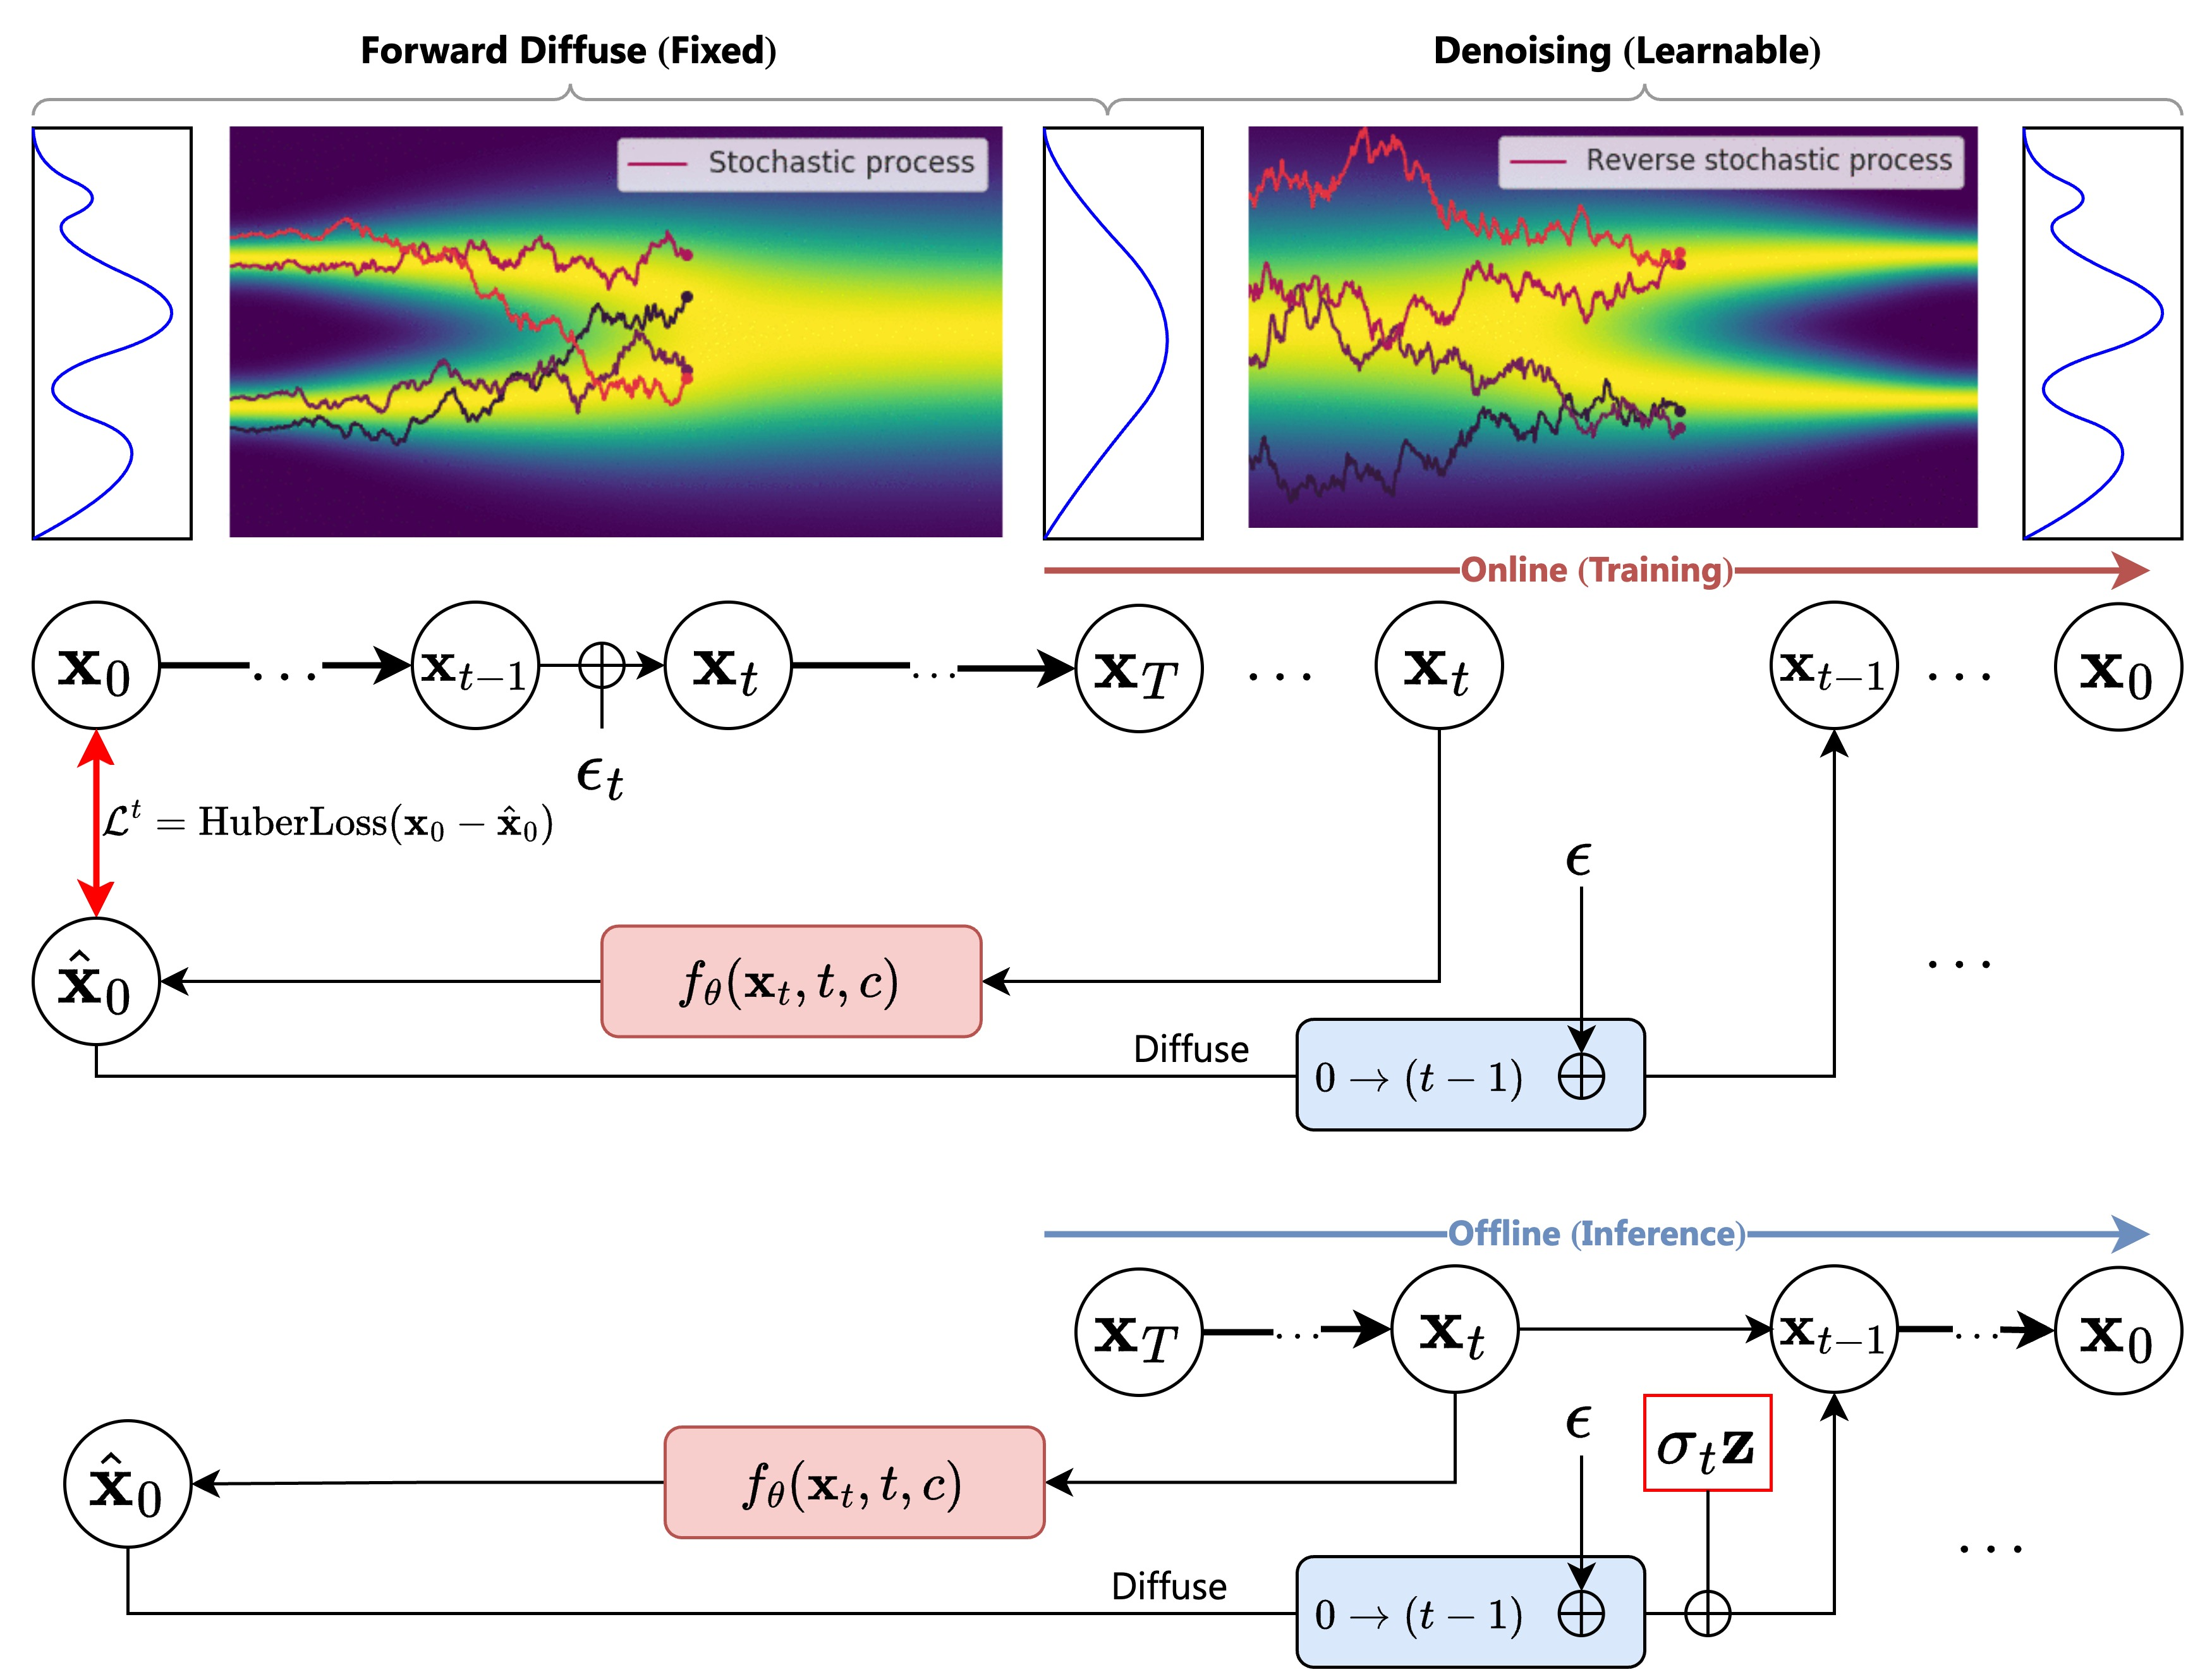
\includegraphics[width=\linewidth]{OnlineAndOffline}
	\caption{Offline (Training) and Online (Inference) Phases}
	\label{fig:OnlineAndOffline}
\end{figure}

To generate gestures of arbitrary length, the original sequence is segmented into clips of length $M$.
During training, the seed gesture can be chosen by randomly selecting a gesture from the dataset or by averaging the clipped segments—here, the mean rotation angles are used.  
Generated frames are processed sequentially, with the last $N=8$ frames taken as the seed for the next iteration.  
For each clip, the gesture $\bx_{t}$ is denoised via $\hat{\bx}_{0} = G_{\theta'}(\bx_{t}, t, c)$; noise is re-added to obtain $\bx_{t-1}$, and the procedure repeats until $t=1$, yielding $\bx_{0}$.

\begin{algorithm}[H]
	\caption{Sampling in OHGesture}
	\label{alg:sampling}
	\setlength{\baselineskip}{10pt}
	\begin{enumerate}
		\item Initialize with noise: $\mathbf{x}_T \sim \mathcal{N}(0, \mathbf{I})$.
		\item Retrieve $\sqrt{\alpha_t}$, $\sqrt{1 - \alpha_t}$, and $\sqrt{\bar{\alpha}_t}$ from training; precompute $\sigma_t$ from $\alpha_t$ for each timestep $t: 1 \rightarrow T$.
		\item Split each 4-second speech segment into $\mathbf{a} \in \mathbb{R}^{64000}$.  
		      The initial seed gesture $\mathbf{s}$ is the data mean and is later updated from the inferred gesture segment.  
		      Select the desired emotion, obtain the transcript $\mathbf{v}$ from speech $\mathbf{a}$, and form the condition $c = [\mathbf{s}, \mathbf{e}, \mathbf{a}, \mathbf{v}]$.
		\item For each timestep, take $t$ \textbf{sequentially} from $[T, \dots, 1]$.
		\item Sample random noise $\mathbf{z} \sim \mathcal{N}(0, \mathbf{I})$.
		\item Infer $\hat{\mathbf{x}}_0^{(t)} = G_{\theta'}(\mathbf{x}_t, t, c)$.
		\item Diffuse $\hat{\mathbf{x}}_0^{(t)}$ from step $0 \rightarrow t$ to obtain $\hat{\mathbf{x}}_{t-1}^{(t)}$.
		\item Add noise: $\hat{\mathbf{x}}_{t-1} = \hat{\mathbf{x}}_{t-1}^{(t)} + \sigma_t \mathbf{z}$.
		\item Return to step 4.  
		      When $t = 1$, output the denoised gesture $\hat{\mathbf{x}}_0$.
	\end{enumerate}
\end{algorithm}

\autoref{alg:sampling} starts by initializing the noisy gesture $\mathbf{x}_T$ from $\mathcal{N}(0, \mathbf{I})$.  
The values $\sqrt{\alpha_t}$, $\sqrt{1-\alpha_t}$, and $\sqrt{\bar{\alpha}_t}$ obtained during training, together with $\sigma_t$, are employed at each timestep (1 … $T$).  
Each 4-second speech segment is represented by $\mathbf{a}$, and the seed gesture $\mathbf{s}$ is taken as the data mean or from the previously inferred segment.  
The desired emotion and the transcript form the condition $c = [\mathbf{s}, \mathbf{e}, \mathbf{a}, \mathbf{v}]$.  
The algorithm proceeds sequentially from $T$ to 1: random noise $\mathbf{z}$ is generated, the model predicts $\hat{\mathbf{x}}_0^{(t)}$ from $\mathbf{x}_t$, $t$, and $c$, then $\hat{\mathbf{x}}_{t-1}^{(t)}$ is computed and updated with noise.  
This loop continues until $t=1$, after which the algorithm outputs the final denoised gesture $\hat{\mathbf{x}}_0$.
